%% For double-blind review submission, w/o CCS and ACM Reference (max submission space)
\documentclass[sigplan,review=false,anonymous=false]{acmart}\settopmatter{printfolios=true,printccs=false,printacmref=false}
\renewcommand\footnotetextcopyrightpermission[1]{}
\pagestyle{plain}
\usepackage{flushend}
%% For double-blind review submission, w/ CCS and ACM Reference
%\documentclass[sigplan,review,anonymous]{acmart}\settopmatter{printfolios=true}
%% For single-blind review submission, w/o CCS and ACM Reference (max submission space)
%\documentclass[sigplan,review]{acmart}\settopmatter{printfolios=true,printccs=false,printacmref=false}
%% For single-blind review submission, w/ CCS and ACM Reference
%\documentclass[sigplan,review]{acmart}\settopmatter{printfolios=true}
%% For final camera-ready submission, w/ required CCS and ACM Reference
%\documentclass[sigplan]{acmart}\settopmatter{}


%% Conference information
%% Supplied to authors by publisher for camera-ready submission;
%% use defaults for review submission.

%\acmConference[]{Workshop on Approximate Computing Across the Stack}
%\acmYear{2018}
%\acmISBN{978-x-xxxx-xxxx-x/YY/MM}
%\acmDOI{10.1145/nnnnnnn.nnnnnnn}
%\startPage{}

%% Copyright information
%% Supplied to authors (based on authors' rights management selection;
%% see authors.acm.org) by publisher for camera-ready submission;
%% use 'none' for review submission.
\setcopyright{none}
%\setcopyright{acmcopyright}
%\setcopyright{acmlicensed}
%\setcopyright{rightsretained}
%\copyrightyear{}           %% If different from \acmYear

%% Bibliography style
\bibliographystyle{ACM-Reference-Format}
%% Citation style
%\citestyle{acmauthoryear}  %% For author/year citations
%\citestyle{acmnumeric}     %% For numeric citations
%\setcitestyle{nosort}      %% With 'acmnumeric', to disable automatic
                            %% sorting of references within a single citation;
                            %% e.g., \cite{Smith99,Carpenter05,Baker12}
                            %% rendered as [14,5,2] rather than [2,5,14].
%\setcitesyle{nocompress}   %% With 'acmnumeric', to disable automatic
                            %% compression of sequential references within a
                            %% single citation;
                            %% e.g., \cite{Baker12,Baker14,Baker16}
                            %% rendered as [2,3,4] rather than [2-4].


%%%%%%%%%%%%%%%%%%%%%%%%%%%%%%%%%%%%%%%%%%%%%%%%%%%%%%%%%%%%%%%%%%%%%%
%% Note: Authors migrating a paper from traditional SIGPLAN
%% proceedings format to PACMPL format must update the
%% '\documentclass' and topmatter commands above; see
%% 'acmart-pacmpl-template.tex'.
%%%%%%%%%%%%%%%%%%%%%%%%%%%%%%%%%%%%%%%%%%%%%%%%%%%%%%%%%%%%%%%%%%%%%%


%% Some recommended packages.
\usepackage{booktabs}   %% For formal tables:
                        %% http://ctan.org/pkg/booktabs
\usepackage{subcaption} %% For complex figures with subfigures/subcaptions
                        %% http://ctan.org/pkg/subcaption
\usepackage{lmodern}
\usepackage{graphicx}
\usepackage{float}
\usepackage{subcaption}
\graphicspath{ {images/} }

\begin{document}

%% Title information
\title{Exploring Floating-Point Trade-Offs in ML}         %% [Short Title] is optional;
                                        %% when present, will be used in
                                        %% header instead of Full Title.
%\titlenote{Both Vanilla and Average variants of the Perceptron algorithm}             %% \titlenote is optional;
                                        %% can be repeated if necessary;
                                        %% contents suppressed with 'anonymous'
%\subtitle{Subtitle}                     %% \subtitle is optional
%\subtitlenote{with sudddddbtitle note}       %% \subtitlenote is optional;
                                        %% can be repeated if necessary;
                                        %% contents suppressed with 'anonymous'


%% Author information
%% Contents and number of authors suppressed with 'anonymous'.
%% Each author should be introduced by \author, followed by
%% \authornote (optional), \orcid (optional), \affiliation, and
%% \email.
%% An author may have multiple affiliations and/or emails; repeat the
%% appropriate command.
%% Many elements are not rendered, but should be provided for metadata
%% extraction tools.

%% Author with single affiliation.
\author{Rocco Salvia}
%\authornote{with author1 note}          %% \authornote is optional;
                                        %% can be repeated if necessary
\orcid{nnnn-nnnn-nnnn-nnnn}             %% \orcid is optional
\affiliation{
  %\position{Position1}
  %\department{Department1}              %% \department is recommended
  \institution{School of Computing, University of Utah, USA}            %% \institution is required
  %\streetaddress{Street1 Address1}
  %\city{City1}
  %\state{State1}
  %\postcode{Post-Code1}
  %\country{Country1}                    %% \country is recommended
}
\email{rocco@cs.utah.edu}          %% \email is recommended

%% Author with two affiliations and emails.
\author{Zvonimir Rakamari\'c}
%\authornote{with author2 note}          %% \authornote is optional;
                                        %% can be repeated if necessary
\orcid{nnnn-nnnn-nnnn-nnnn}             %% \orcid is optional
\affiliation{
  %\position{Position2a}
  %\department{Department2a}             %% \department is recommended
  \institution{School of Computing, University of Utah, USA}
  %% \institution is required
  %\streetaddress{Street2a Address2a}
  %\city{City2a}
  %\state{State2a}
  %\postcode{Post-Code2a}
  %\country{Country2a}                   %% \country is recommended
}
\email{zvonimir@cs.utah.edu}         %% \email is recommended


%% Abstract
%% Note: \begin{abstract}...\end{abstract} environment must come
%% before \maketitle command
\begin{abstract}
Perceptron and Support Vector Machine (SVM) algorithms are two well-known linear predictors. They are used to compute a hypothesis function given the labeled training data to predict labels of unknown samples in the future. 
Both training and testing procedures are typically implemented using double precision floating-points to minimize the error, which often results in overly conservative implementations that waste runtime and/or energy. 
In this work, we empirically analyze the impact of floating-point precision on these predictors. We assess whether the precision of reading the dataset, training, or testing is the most important for the overall accuracy.
Our analysis in particular focuses on very small floating-point bit-widths (i.e., only several bits of precision), and compares these against the well-known and widely used single and double precision types.
\end{abstract}


%% 2012 ACM Computing Classification System (CSS) concepts
%% Generate at 'http://dl.acm.org/ccs/ccs.cfm'.
%\begin{CCSXML}
%<ccs2012>
%<concept>
%<concept_id>10011007.10011006.10011008</concept_id>
%<concept_desc>Software and its engineering~General programming languages</concept_desc>
%<concept_significance>500</concept_significance>
%</concept>
%<concept>
%<concept_id>10003456.10003457.10003521.10003525</concept_id>
%<concept_desc>Social and professional topics~History of programming languages</concept_desc>
%<concept_significance>300</concept_significance>
%</concept>
%</ccs2012>
%\end{CCSXML}

%\ccsdesc[500]{Software and its engineering~General programming languages}
%\ccsdesc[300]{Social and professional topics~History of programming languages}
%% End of generated code
%% Keywords
%% comma separated list
%\keywords{SVM, Perceptron, floating-point, consumption.}  %% \keywords are mandatory in final camera-ready submission
%% \maketitle
%% Note: \maketitle command must come after title commands, author
%% commands, abstract environment, Computing Classification System
%% environment and commands, and keywords command.
\maketitle
\section{Introduction}
Floating-point representation was invented to model real numbers in computers. Representing real numbers as a finite sequence of bits naturally introduces approximation, which leads to errors in computations~\cite{WhatEvery}. 
Hence, developers are often conservative about floating-point precision, and use the maximum precision provided by their target platform. However, executing floating-point operations can be a major contributor to runtime and energy consumption. For example, Tagliavini et al.~\cite{softfloat} run a set of floating-point applications on a microcontroller, and empirically show that 30\% of the energy consumption was due to floating-points computations and another 20\% due to moving operands between memory and registers.
Hence, leveraging lower precisions can lead to significant savings, and the impact of low-cost floating-point precisions on machine learning predictors is an active research area.

Several recent papers explore the effects of floating-point and fixed precision reduction on neural networks~\cite{gupta,dorefa,Hubara}. Typically, they conclude that using very low precision arithmetic results in minimal loss of accuracy compared to single or double precision.
%Gupta et al.\cite{gupta} prove that deep neural network can be trained using low precision fixed-point arithmetic, with a minimal sacrifice of quality. 
%They show how performing fixed point arithmetic using only 16-bit of precision produces same results of IEEE 754 single floating-point representation (32-bit precision). 
%Zhou et al. \cite{dorefa} propose innovative methods to train Convolutional-Neural-Networks (CNNs) with low bit-width weights, activations and gradients. They show how using 1-bit weight, 1-bit activation and 2-bit gradient achieve a value of 93\% of accuracy compared to 97\% obtained with 32-bit single precision. 
%Hubara et al.\cite{Hubara} introduce a method to train Quantized-Neural-Networks (QNNs) using low precision arithmetic.
%They showed how using 4 bits for weights and activation step result in a degradation of 5.5\% compared to 32-bit single precision.
Others studied the effects of reduced precision on the misprediction rate of the SVM algorithm, and
focused on the quantization of the classification process~\cite{auguita,SVM}.


In this work, we study the effects of floating-point precision on the accuracy
of the Perceptron and SVM machine learning algorithms.  We implemented the
algorithms using multiple-precision numerical libraries, which allows us to
independently vary the precision of reading the dataset, computing the model,
and testing of the computed model. We empirically evaluated the
precision/accuracy trade-offs on several datasets, with a particular focus on
very small floating-point bit-widths.  Our results and conclusions serve as a
guideline for making floating-point precision choices when implementing these
algorithms.

%Our approach is similar because the analysis applies only on mantissa tuning, on the other hand they focus the quantization on the classification process, without taking in consideration both training and reading phases of the algorithm. In this way they do not consider all the dependencies among reading, computing and testing. Moreover, it is not clear what is the precision used for reading during testing. 
%We detect the best hyperparameter configuration for each dataset before performing any quantization, while the authors adopts the same configuration for all the datasets.
%Although their implementation of SVM differs from our (Gaussian and Linear Kernel), they empirically show that using any precision in the range [52,15] results in same accuracy. 
%At the same time, we are aware of many analyzers that are able to scan a black box algorithm to minimize the precision of each floating-point instruction while still maintaining the desired value of accuracy \cite{reducelam}\cite{mixpreclam}\cite{precimonious}\cite{blame}. 

%Program analysis applied to floating-point instructions usually maintains few 'ghosts' executions of the program, to replicate the behavior of it with different floating-point precisions.\cite{blame}\cite{precimonious}. Once a particular configuration satisfy the evaluation procedure provided by the user, the binary code is altered instructions is injected into the binary code of the program and the candidate result may be evaluated again.\cite{mixpreclam}\cite{reducelam}.

%In particular, the aim of these tools is to produce the minimal configuration of FP instructions such that the output keeps same quality. 
%These techniques involve both static and dynamic approaches: usually the first is used to detect FP instructions in the program, while the second one produces improvement on the configuration of the solution, also due to 'ghost' executions that verify the current configuration.

%Our work admire and look forward these analyzers, but we move away from the detection of the minimal floating-point configuration of Perceptron and SVM. 

%We study what affect the accuracy of these predictors in case of poor floating-point precision computations. Our goal is to empirically show how limited can be the floating-point format while still maintaining high accuracy. Also, we report which step in the lifetime of these predictors is most sensitive to precision tuning. 

%We want to compare the accuracy of these predictors ($\frac{Correct.Prediction}{Tot.Samples}$) between minimal values of floating-point precision (from 2 to 10 bits for mantissa representation) and well known (and expensive) single and double precisions. %


\begin{figure*}
	\hspace*{\fill}%
	\begin{subfigure}[b]{0.29\linewidth}
		%\centering
		\caption{{\tiny{Diabet(AP): 2-bit(t) vs 52-bit(b)}}}
		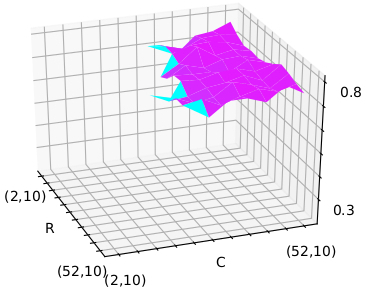
\includegraphics[width=\linewidth, height=0.6\linewidth]{DiabetMPFRpart3APTes2}
	\end{subfigure}
	\hfill%
	\begin{subfigure}[b]{0.29\linewidth}
		%\centering
		\caption{{\tiny{Splice(SVM):7-bit(t) vs 52-bit(b)}}}
		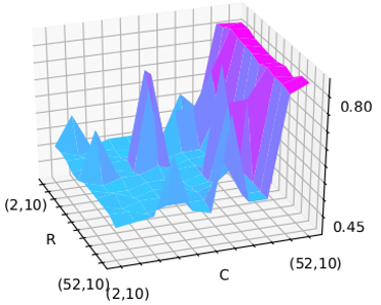
\includegraphics[width=\linewidth, height=0.6\linewidth]{SpliceMPFRpart4SVMTest7}
	\end{subfigure}
	\hfill%
	\begin{subfigure}[b]{0.29\linewidth}
		\caption{{\tiny{Heart(SVM):3-bit(t) vs 52-bit(b)}}}
		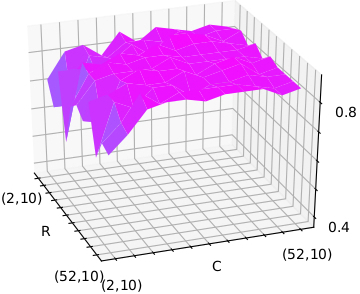
\includegraphics[width=\linewidth, height=0.6\linewidth]{heartFLEXpart3SVMTest3}
	\end{subfigure}
	\hspace*{\fill}%  
	%\caption{General caption}
\end{figure*}
\setcounter{figure}{0}    
\begin{figure*}
	\hspace*{\fill}%
	\begin{subfigure}[b]{0.29\linewidth}
		\centering
		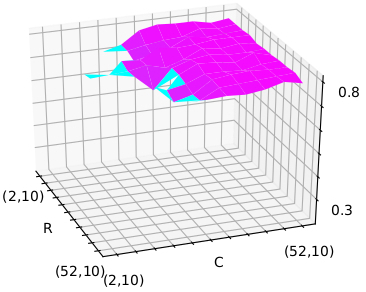
\includegraphics[width=\linewidth, height=0.6\linewidth]{DiabetMPFRpart3APTes52}
		%\caption{Lorem Ipsum is simply dummy text of the printing and} %typesetting industry. Lorem Ipsum has been the industry's standard dummy text ever since the 1500s, when an unknown printer took a galley of type and scrambled it to make a type specimen book.}
	\end{subfigure}\hfill%
	\begin{subfigure}[b]{0.29\linewidth}
		\centering
		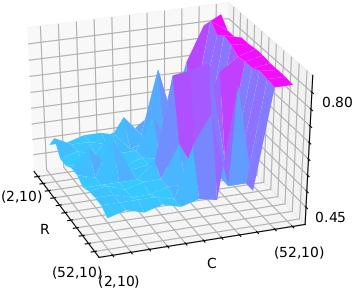
\includegraphics[width=\linewidth, height=0.6\linewidth]{SpliceMPFRpart4SVMTest52}
		%\caption{Lorem Ipsum is simply dummy text of the printing and}
		%typesetting industry. Lorem Ipsum has been the industry's standard dummy text ever since the 1500s, when an unknown printer took a galley of type and scrambled it to make a type specimen book.}
	\end{subfigure}\hfill%
	\begin{subfigure}[b]{0.29\linewidth}
		\centering
		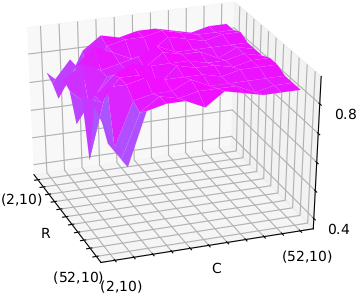
\includegraphics[width=\linewidth, height=0.6\linewidth]{heartFLEXpart3SVMTest52}
		%\caption{Lorem Ipsum is simply dummy text of the printing} 
		%and typesetting industry. Lorem Ipsum has been the industry's standard dummy text ever since the 1500s, when an unknown printer took a galley of type and scrambled it to make a type specimen book.}{\tiny }
	\end{subfigure}
	\hspace*{\fill}%
	\caption{Accuracy for various precision regimes. Graphs compare two chosen testing precisions (top and bottom) on different datasets. Axis $R$ denotes reading precision, $C$ computing precision, and the third axis shows the accuracy. For example, $(2,10)$ represents a 2-bit mantissa and 10-bit exponent.}
	\label{results}
\end{figure*}


\section{Methodology}

The format adopted for floating-point representation consists of the sign of the number, significand (mantissa), and exponent. 
This format is part of the IEEE 754 standard~\cite{IEEE}, which includes, among others, two well-known and popular representations: single precision (1-bit sign, 23-bit mantissa, 8-bit exponent) and double precision (1-bit sign, 52-bit mantissa, 11-bit exponent).
However, it has been shown that using representations other than these default ones can be beneficial in many applications to improve runtime and energy efficiency~\cite{softfloat}, which is what we explore in this work.
%It has been showed \cite{softfloat} the way mantissa and exponent split the total amount of bits in single and double representation can be further improved.

The Perceptron algorithm~\cite{perceptron} is a supervised learning algorithm.
It is a mistake-driven algorithm: once a sample is misclassified the predictor is updated. The update step involves the weight vector, which is the main contributor to the classification process. 
%The Perceptron is composed of one neuron with activation function.
Particularly interesting in terms of floating-point analysis is the average variant of Perceptron, which
maintains an average predictor weighted on wrong predictions, and it needs a wider dynamic range for this computation.

The SVM algorithm~\cite{cortes,vapnik} also produces a linear classifier, but it differs from Perceptron in the way the hyperplane is obtained. It is more restrictive than Perceptron since it aims for a safe margin between the linear separator and the closest samples. 
%We implemented the soft version of SVM, meaning that samples are allowed to exist between the linear separator and the margin. 
SVM is trained using a stochastic sub-gradient descent method, whose goal is to maximize the safe margin while minimizing the number of samples violating it.



We implemented Perceptron (P), Average Perceptron (AP), and SVM algorithms using
multiple-precision numerical libraries MPFR~\cite{MPFR} and
FlexFloat~\cite{softfloat}.
%such that each floating-point instruction can be bounded by a desired floating-point format.
This allows us to specify how many bits are assigned to mantissa and exponent of each floating-point instruction.
%As a result, our analysis spans lowest format configurations allowed for mantissa representation.
%In case of exception (only for lack of dynamic range, a lack of precision for mantissa never produces exception) the procedure is stopped, the exponent is increased, and the algorithm starts again.
We mainly focus on varying the mantissa bits, since exponent does not play a
major role in influencing the accuracy once it is large enough that exceptions
(e.g., overflow, underflow) do not appear.


We analyze the accuracy impact of precision of the three main learning
algorithm stages: reading the dataset, training, and testing.
%The goal is to detect which dependencies exist between them. 
%We want to stress the combinations of formats used for representations.
%The first goal of our work is to detect a minimum threshold in the precision to adopt for the dataset storing. 
Storing and reading the dataset in low precision potentially leads to savings in memory traffic.
%The first goal of out work is to minimize the storage format of the dataset.
%Minimizing this precision, while still maintaining high values for the accuracy of predictors ($\frac{Correct.Classifications}{Tot.Classifications}$) results in enormous saving in terms of architecture complexity, energy consumption, computational effort, and storage space\cite{softfloat}.
%We call this parameter: \emph{dataset precision}.
Once the dataset is read at the desired floating-point precision, the training
procedure of an algorithm executes with the specified computing precision.
Finally, the generated model is passed to the testing procedure,
executed with the specified testing precision.
We measure the accuracy of the model by performing a 4-fold cross-validation on each dataset.



\section{Results}

We used the following five datasets for our empirical evaluation: \emph{fourclass}~\cite{fourclass}, \emph{heart}, \emph{diabet}, \emph{ionosphere}, and \emph{splice}~\cite{UCI}.
They range in size between 270--1000 samples and 2--60 features.
Before training, we scale each dataset to the interval $[-1,1]$, and detect a
good hyper-parameters configuration for each algorithm.
We vary the number of mantissa bits for reading, training, and testing in the range 
$[2,3,\ldots,9,10,23,52]$.
We made the source code and detailed results publicly available.\footnote{See \url{https://github.com/soarlab/FPML}}
%All tests are performed on a PC desktop machine.
%running Ubuntu 16.04 i7-6700HQ CPU @ 2.60GHz and 16GB RAM.
%All the graphs are obtained with matplotlib library\cite{matplotlib}. 
%
Figure~\ref{results} shows several representative and interesting graphs we generated,
and in the rest of this section we discuss several key observations.

The precision used to store and read the dataset can be substantially reduced
with respect to single or double precisions. This is encouraging since
detecting a minimal threshold value for the reading precision can significantly
reduce memory traffic.  In all our datasets, reducing the reading precision
does not have a noticeable impact on the final accuracy --- samples can be
stored even using only 3 bits for mantissa.

The computing precision is the most critical and sensitive parameter. For
example, Figure~\ref{results}(b) shows that in case of the \emph{Splice}
dataset, SVM has to be trained at the highest (double) precision to achieve
good accuracy.  To summarize, out of 10 analysis runs (5 AP and 5 SVM) only
30\% of the time training has to be performed at double precision, while in the
rest 10 bits is enough.  (Note that we excluded Perceptron from the summary
because it is hard to observe a precision threshold due to its erratic behavior
in terms of accuracy.)

The testing precision can often be substantially reduced without having a major
impact on the accuracy.
For our five datasets, using 9 bits mantissa for testing is always enough to
reach the same accuracy as double precision. More precisely, 60\% of the time 6 bits
is enough, while 30\% of the time 4 bits is enough.
Finally, in one case using only 2 bits for testing achieves similar accuracy
as double precision.
Figures~\ref{results}(a,c) show how testing with just 2 and
3 bits produces accuracy similar to using double (52 bits).
This is particularly important for deployment scenarios where training is
performed on large machines potentially using double precision, but the learned
models are deployed to for example mobile platforms using very low precision to
conserve energy.

\paragraph{Acknowledgements}
We thank Annie Cherkaev and Vi\-vek Srikumar for insightful discussions. This
work was supported in part by NSF CCF 1552975.

	%, but it requires an higher \emph{computing precision} (purple region is restricted on top graph).
	%Figure(\textbf{c}) shows how testing with 3-bit produces similar accuracy of 52-bit. 
	%Moreover, the following configuration: reading with 2-bit, training with 6-bit, and testing with 3-bit is enough to reach similar accuracy of "all" double configuration.

%% Acknowledgments
%\begin{acks}                            %% acks environment is optional
%                                        %% contents suppressed with 'anonymous'
%  %% Commands \grantsponsor{<sponsorID>}{<name>}{<url>} and
%  %% \grantnum[<url>]{<sponsorID>}{<number>} should be used to
%  %% acknowledge financial support and will be used by metadata
%  %% extraction tools.
%  This material is based upon work supported by the
%  \grantsponsor{GS100000001}{National Science
%    Foundation}{http://dx.doi.org/10.13039/100000001} under Grant
%  No.~\grantnum{GS100000001}{nnnnnnn} and Grant
%  No.~\grantnum{GS100000001}{mmmmmmm}.  Any opinions, findings, and
%  conclusions or recommendations expressed in this material are those
%  of the author and do not necessarily reflect the views of the
%  National Science Foundation.
%\end{acks}


%% Bibliography
\bibliography{bibfile}


%% Appendix
%\appendix
%\section{Appendix}
%
%Text of appendix \ldots

\end{document}
